\chapter{পূর্বাভাসমূলক মডেলিং ও মূল্যায়ন}\label{ch:models}

এই অধ্যায় পূর্বাভাসমূলক প্রশ্ন, \emph{সামনে কী ঘটতে পারে?}, এর উত্তর দেয়। এখানে পর্যায়ক্রমে চারটি বিশ্লেষণী সমস্যা আলোচিত: চাহিদা
পূর্বাভাস, বড় অর্ডারের ক্লাসিফিকেশন, বিভাজন এবং অ্যানোমালি ডিটেকশন।

\section{মাসিক চাহিদা পূর্বাভাস}
\subsection{প্রস্তুতি}
পূর্বাভাস প্যানেলে মাসিকভাবে পর্যবেক্ষিত \PanelSeries টি পণ্য রয়েছে। প্রশিক্ষণ-সারি \PanelTrain টি (2020--2024) এবং পরীক্ষা-সারি
\PanelTest টি (জানুয়ারি 2025 -- সেপ্টেম্বর 2026)। প্রতিটি মডেল $\log(1+\text{units})$ পূর্বাভাস করে, যা পরে ইউনিটে রূপান্তরিত হয়।
Log স্কেল চাহিদার গুণাত্মক প্রকৃতির সঙ্গে মানানসই এবং সবচেয়ে বড় পণ্যগুলোকে fit-এ আধিপত্য করতে দেয় না। সাতটি অ্যালগরিদম
\cref{ch:method}-এ বর্ণিত expanding-window ভাঁজে randomised search দিয়ে টিউন করা হয়েছে; নির্বাচিত hyper-parameter
\cref{app:hyper}-এর \cref{tab:hyper}-এ দেওয়া আছে।

\subsection{এক-ধাপ-অগ্রিম ফলাফল}
\Cref{tab:forecast} পরীক্ষাকালের কর্মদক্ষতা দেখায় যখন প্রতিটি মাস আগের মাস পর্যন্ত প্রকৃত ইতিহাস দিয়ে পূর্বাভাস করা হয়, অর্থাৎ মাসিক
পরিকল্পনা-চক্রের বাস্তব পরিস্থিতি। প্রতিটি মেশিন লার্নিং মডেল দুটি naive বেঞ্চমার্ককেই স্পষ্টভাবে হারিয়েছে। সেরা মডেল \BestReg-এর
RMSE \BestRegRMSE ইউনিট, WAPE \BestRegWAPE\% এবং $R^2=\BestRegRtwo$; অর্থাৎ seasonal-naive নিয়মের (\SNaiveRMSE) চেয়ে RMSE
\GainVsSNaive\% কম এবং naive নিয়মের (\NaiveRMSE) চেয়ে \GainVsNaive\% কম।

\begin{table}[htbp]
\centering
\footnotesize
\caption{মাসিক পণ্য-চাহিদা পূর্বাভাস: পরীক্ষাকালের কর্মদক্ষতা (এক-ধাপ-অগ্রিম, জানুয়ারি 2025--সেপ্টেম্বর 2026)}
\label{tab:forecast}
\begin{adjustbox}{max width=\linewidth}
\begin{tabular}{lrrrrrrrr}
\toprule
\textbf{Model} & \textbf{MAE} & \textbf{MSE} & \textbf{RMSE} & \textbf{R$^2$} & \textbf{MAPE \%} & \textbf{WAPE \%} & \textbf{CV RMSE} & \textbf{Fit (s)} \\
\midrule
Seasonal naive (same month last year) & 120.0 & 23,233 & 152.4 & 0.551 & 15.38 & 14.74 & -- & 0.0 \\
Naive (last month) & 139.8 & 31,051 & 176.2 & 0.400 & 18.00 & 17.17 & -- & 0.0 \\
Support Vector Regression & 90.6 & 13,271 & 115.2 & 0.744 & 12.26 & 11.13 & 0.2151 & 20.0 \\
Linear Regression & 91.3 & 13,861 & 117.7 & 0.732 & 11.48 & 11.21 & 0.1691 & 0.4 \\
XGBoost & 93.3 & 14,294 & 119.6 & 0.724 & 12.28 & 11.46 & 0.1917 & 103.3 \\
Random Forest & 93.0 & 14,413 & 120.1 & 0.722 & 12.04 & 11.42 & 0.1918 & 142.2 \\
Gradient Boosting & 95.7 & 15,113 & 122.9 & 0.708 & 12.51 & 11.76 & 0.1889 & 108.6 \\
K-Nearest Neighbors & 97.0 & 15,865 & 126.0 & 0.694 & 12.01 & 11.91 & 0.1951 & 8.4 \\
Decision Tree & 103.6 & 17,978 & 134.1 & 0.653 & 13.70 & 12.73 & 0.2077 & 7.2 \\
\bottomrule
\end{tabular}
\end{adjustbox}
\par\smallskip\parbox{0.92\linewidth}{\footnotesize\emph{টীকা:} ত্রুটি প্রতি পণ্য-মাসে ইউনিটে। CV RMSE হলো টিউনিংয়ে ব্যবহৃত 2022, 2023 ও 2024-এর expanding-window ভাঁজে log স্কেলে গড় validation RMSE। বেসলাইনের কোনো fitting লাগে না।}
\end{table}

আরও তিনটি পর্যবেক্ষণ উল্লেখযোগ্য। প্রথমত, ভালো মডেলগুলোর পার্থক্য সামান্য: RMSE \BestRegRMSE থেকে \WorstRegRMSE ইউনিটের মধ্যে,
এবং log-ফিচারে linear regression (\LinRMSE) tree ensemble-এর (random forest \RFRMSE, XGBoost \XGBRMSE) সঙ্গে প্রতিযোগিতামূলক।
ভালো lag ও মৌসুমি ফিচার থাকলে সমস্যাটি মূলত log-linear হয়ে যায়, ফলে মডেলের জটিলতা সামান্যই যোগ করে; এটি
\citet{makridakis2018}-এর সঙ্গে সামঞ্জস্যপূর্ণ। দ্বিতীয়ত, একক decision tree সবচেয়ে দুর্বল (\DTRMSE), যা এর উচ্চ ভেদাঙ্কের কারণে
প্রত্যাশিত; একটি forest-এ অনেক tree-র গড় নিলে এই দুর্বলতার বেশিরভাগ দূর হয় \citep{breiman2001}। তৃতীয়ত, প্রশিক্ষণ-বছরের
cross-validated স্কোর মডেলগুলোকে পরীক্ষা-স্কোরের মতোই ক্রমে সাজায়, তাই যাচাই-নকশাটি ভবিষ্যৎ কর্মদক্ষতার নির্ভরযোগ্য নির্দেশক।
\Cref{fig:forecastcomp} মডেলগুলোর তুলনা করে এবং দেখায় যে ভিন্ন আকারের পণ্যেও \BestReg-এর পূর্বাভাস প্রকৃত মানের খুব কাছাকাছি।

\begin{figure}[htbp]\centering
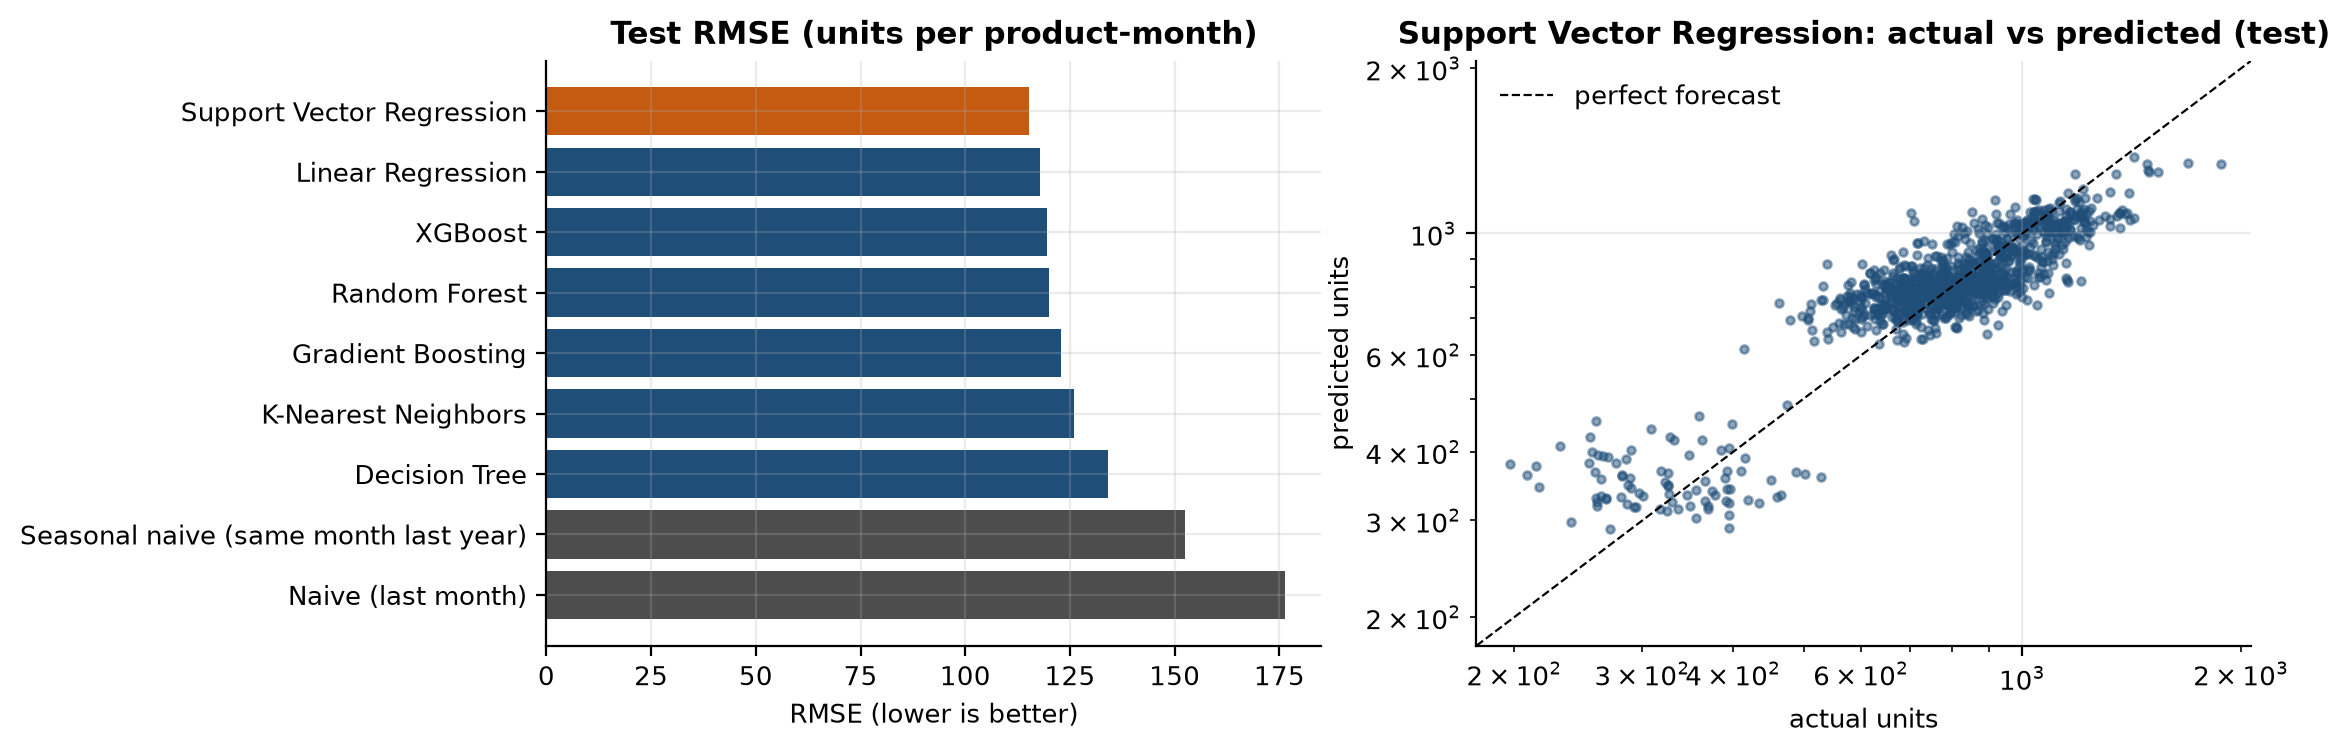
\includegraphics[width=\linewidth]{ml_forecast_comparison}
\caption{সব পূর্বাভাস মডেলের পরীক্ষা-RMSE (বামে; সেরা মডেল চিহ্নিত, বেসলাইন ধূসর) এবং সেরা মডেলের প্রকৃত বনাম পূর্বাভাসিত ইউনিট (ডানে)}\label{fig:forecastcomp}
\end{figure}

\subsection{Recursive বহু-ধাপ ফলাফল}
একটি কঠিনতর পরীক্ষা হলো ডিসেম্বর 2024 থেকে প্রশিক্ষণের পরে কোনো প্রকৃত ডেটা \emph{না দেখে} সব 21টি পরীক্ষা-মাসের পূর্বাভাস দেওয়া,
যেখানে প্রতিটি মাসের পূর্বাভাস পরের মাসের ইতিহাস হিসেবে ফিরে আসে; এটি বার্ষিক বাজেটের পরিস্থিতি। \Cref{tab:recursive} দেখায় যে সেরা
মডেলগুলোর অবনতি সামান্য: \BestRec-এর WAPE \BestRecWAPE\% ($R^2=\BestRecRtwo$), যা 2024-এর প্যাটার্ন পুনরাবৃত্তির চেয়ে অনেক ভালো।
Recursion-এ XGBoost-এর অবনতি সবচেয়ে বেশি: যখন মডেলের নিজের পূর্বাভাস ইনপুট হয় তখন ত্রুটি জমা হয়, এবং প্রশিক্ষণ ডেটায় ঘনিষ্ঠভাবে
fit করা boosted tree এতে বেশি ক্ষতিগ্রস্ত হয়।

\begin{table}[htbp]
\centering
\small
\caption{ডিসেম্বর 2024 থেকে recursive 21-মাসের পূর্বাভাস (প্রশিক্ষণের পরে কোনো প্রকৃত ডেটা ব্যবহৃত হয়নি)}
\label{tab:recursive}
\begin{adjustbox}{max width=\linewidth}
\begin{tabular}{lrrrrr}
\toprule
\textbf{Model} & \textbf{MAE} & \textbf{RMSE} & \textbf{R$^2$} & \textbf{MAPE \%} & \textbf{WAPE \%} \\
\midrule
Random Forest & 91.0 & 117.0 & 0.736 & 11.85 & 11.18 \\
Support Vector Regression & 92.3 & 117.2 & 0.735 & 12.65 & 11.34 \\
Linear Regression & 94.1 & 121.4 & 0.715 & 11.73 & 11.56 \\
XGBoost & 104.1 & 137.5 & 0.635 & 16.17 & 12.79 \\
Seasonal naive (2024 pattern repeated) & 125.9 & 158.1 & 0.517 & 15.87 & 15.47 \\
\bottomrule
\end{tabular}
\end{adjustbox}
\end{table}

\subsection{কোম্পানি-পর্যায়ের পূর্বাভাস ও মডেল মিলকরণ}
পণ্যের পূর্বাভাস যোগ করে কোম্পানির মোট পাওয়া যায়, যা সরাসরি মোট সিরিজে fit করা পরিসংখ্যানিক মডেলের সঙ্গে তুলনা করা যায়
(\cref{tab:company}, \cref{fig:companyfc})। এই সমষ্টিগত পর্যায়ে additive প্রবণতা ও multiplicative মৌসুমিতাসহ Holt--Winters মডেল
সবচেয়ে নির্ভুল, MAPE মাত্র \HWMAPE\%। যোগ করা মেশিন লার্নিং পূর্বাভাসও নির্ভুল, তবে সামান্য কম। এটি সাহিত্যের সঙ্গে সামঞ্জস্যপূর্ণ:
মসৃণ সমষ্টিগত সিরিজে পরিসংখ্যানিক মডেল সুবিধা পায়, আর পৃথক পণ্যের স্তরে মেশিন লার্নিংয়ের সমন্বিত-শিক্ষণ সুবিধা কাজে লাগে। তাই
কাঠামোটি দুটিকে \emph{top-down reconciliation} দিয়ে একত্র করে \citep{athanasopoulos2009}: Holt--Winters কোম্পানির মোট ও তার
পূর্বাভাস-ব্যবধান নির্ধারণ করে, আর মেশিন লার্নিং মডেল সেই মোটকে পণ্যগুলোর মধ্যে বণ্টন করে, যাতে পণ্য-পরিকল্পনা হুবহু কোম্পানি-পরিকল্পনার
সমান হয়।

\begin{table}[htbp]
\centering
\small
\caption{কোম্পানি-স্তরের মাসিক ইউনিট পূর্বাভাস, পরীক্ষাকাল জানুয়ারি 2025--সেপ্টেম্বর 2026}
\label{tab:company}
\begin{adjustbox}{max width=\linewidth}
\begin{tabular}{lrrr}
\toprule
\textbf{Model (company-total monthly units)} & \textbf{MAE} & \textbf{RMSE} & \textbf{MAPE \%} \\
\midrule
Holt-Winters (additive trend, multiplicative season) & 559 & 698 & 1.32 \\
SARIMA(1,1,1)(0,1,1)$_{12}$ on log units & 687 & 806 & 1.65 \\
Support Vector Regression one-step, summed over products & 712 & 875 & 1.68 \\
Random Forest recursive, summed over products & 1,186 & 1,386 & 2.77 \\
Seasonal naive (2024 repeated) & 2,549 & 2,817 & 6.00 \\
\bottomrule
\end{tabular}
\end{adjustbox}
\end{table}

\begin{figure}[htbp]\centering
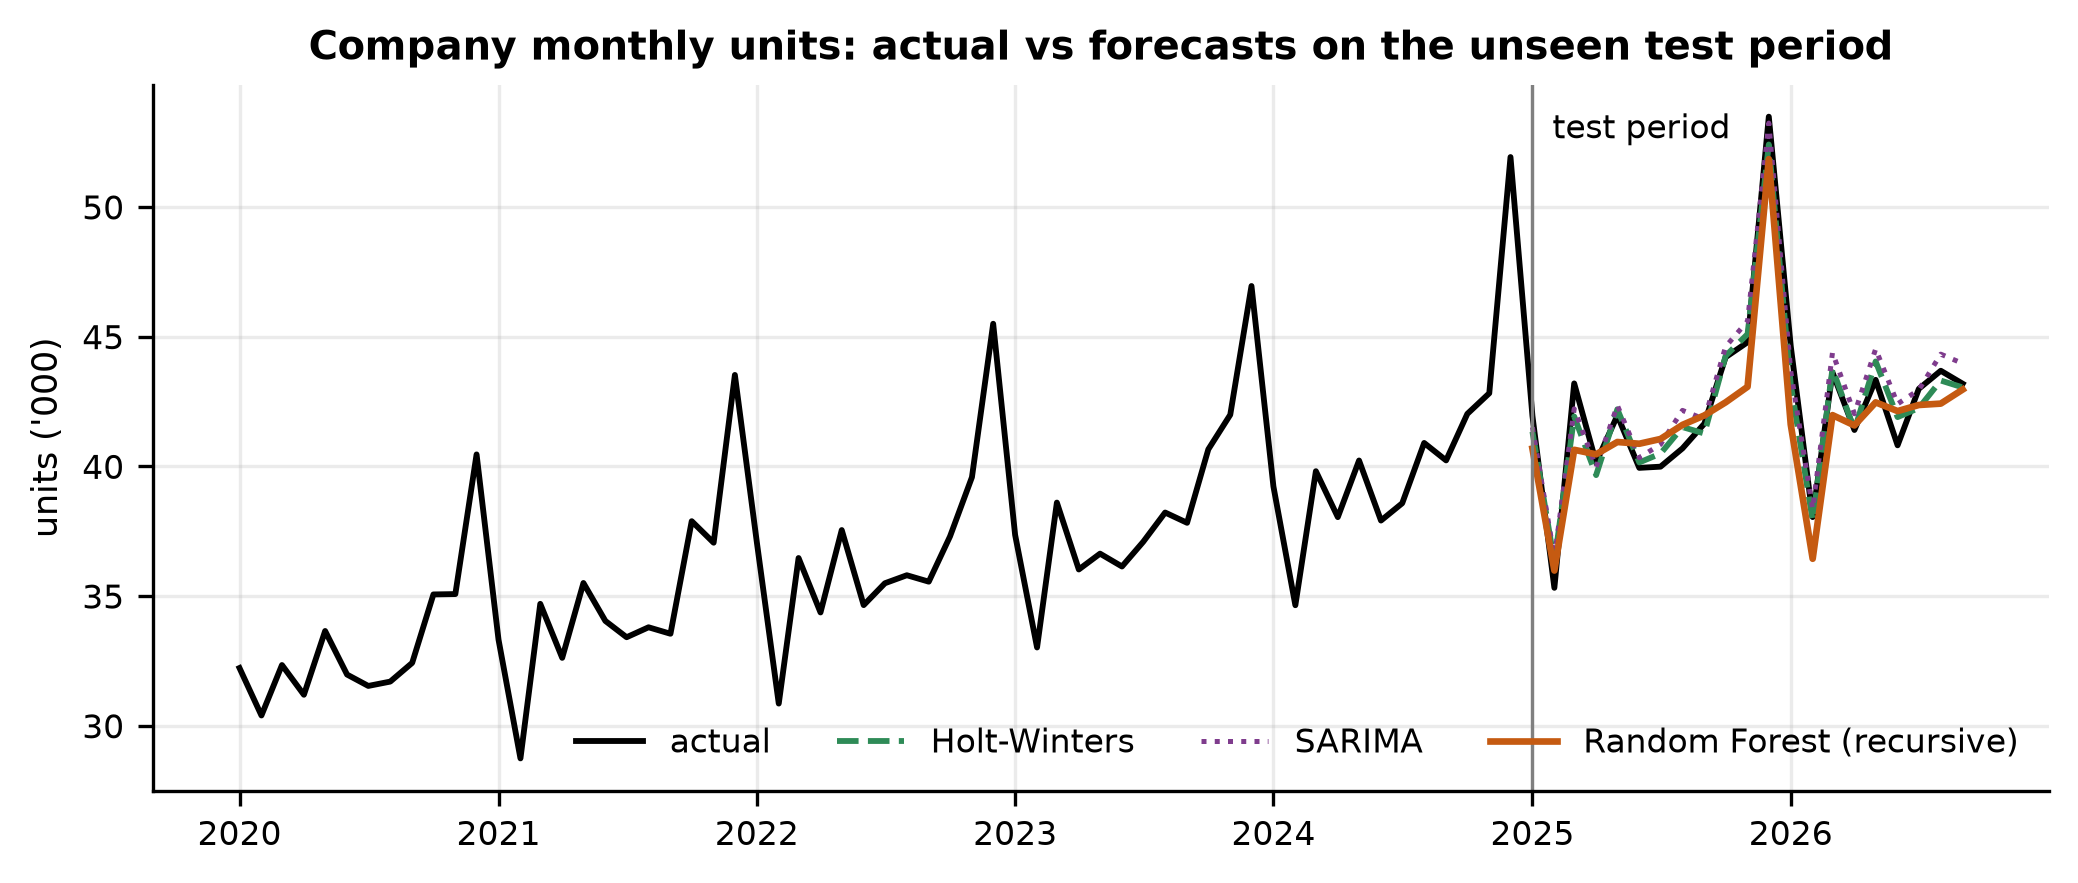
\includegraphics[width=\linewidth]{ml_company_forecast_test}
\caption{কোম্পানির মাসিক ইউনিট: পরীক্ষাকালে প্রকৃত মান ও প্রতিযোগী পূর্বাভাস}\label{fig:companyfc}
\end{figure}

\subsection{পূর্বাভাসের চালিকাশক্তি কী?}
\Cref{fig:importance} মডেলগুলো ব্যাখ্যা করে। \BestReg-এর permutation importance দেখায় যে সাম্প্রতিক ইতিহাস (lag ও rolling গড়)
সবচেয়ে বেশি তথ্য বহন করে, তারপর মৌসুমি ফিচার। XGBoost-এর SHAP মানও একই চিত্র দেয় এবং ডিসেম্বর-সূচক ও 12-মাসের lag-কে তুলে ধরে,
যা মৌসুমি শীর্ষ ধরে। মূল্য-ফিচারের প্রভাব কম, যা \cref{ch:eda}-এর প্রায়-শূন্য স্থিতিস্থাপকতার সঙ্গে মেলে; অর্থাৎ মডেল ও ব্যাখ্যামূলক বিশ্লেষণ
একই গল্প বলে।

\begin{figure}[htbp]\centering
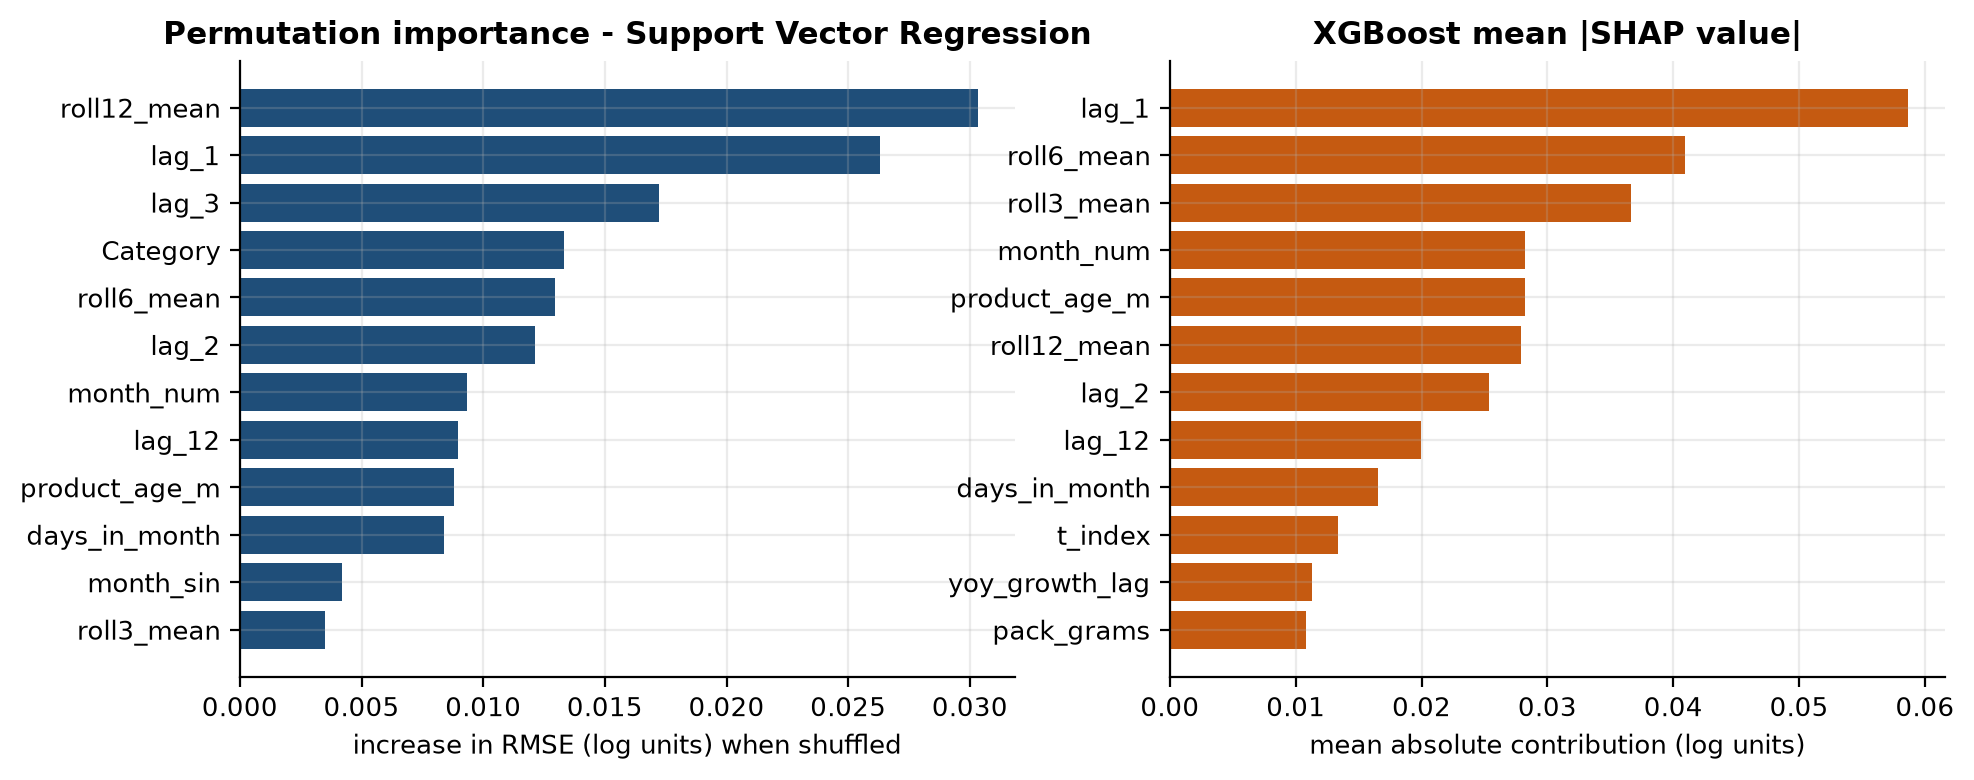
\includegraphics[width=\linewidth]{ml_feature_importance}
\caption{সেরা পূর্বাভাস মডেলের permutation importance (বামে) এবং XGBoost-এর গড় পরম SHAP মান (ডানে)}\label{fig:importance}
\end{figure}

\subsection{বারো মাসের দৃষ্টিভঙ্গি}
নির্বাচিত মডেলগুলো সেপ্টেম্বর 2026 পর্যন্ত সব ডেটায় পুনরায় প্রশিক্ষিত হয়ে অক্টোবর 2026 -- সেপ্টেম্বর 2027-এর পূর্বাভাস দিয়েছে
(\cref{tab:future}, \cref{fig:future})। এই বারো মাসে নিট বিক্রয়ের পূর্বাভাস \FutSales মিলিয়ন টাকা, 80\% ব্যবধান \FutSalesLo থেকে
\FutSalesHi মিলিয়ন, যা আগের বারো মাসের (\PrevSales মিলিয়ন টাকা) চেয়ে \FutGrowth\% বেশি। ইউনিটে পরিবর্তন প্রত্যাশিত \FutUnitsGrowth\%,
এবং ডিসেম্বরের শীর্ষ আবার ফিরবে। পূর্বাভাসে \FutTopCategory সবচেয়ে বড় ক্যাটাগরি থাকছে। এই দৃষ্টিভঙ্গি সরাসরি উৎপাদন, ক্রয় ও বাজেট
প্রক্রিয়ায় ব্যবহার করা যায়।

\begin{table}[htbp]
\centering
\footnotesize
\caption{বারো মাসের অগ্রিম পূর্বাভাস, অক্টোবর 2026 -- সেপ্টেম্বর 2027}
\label{tab:future}
\begin{adjustbox}{max width=\linewidth}
\begin{tabular}{lrrrrrrr}
\toprule
\textbf{Month} & \textbf{Units ML raw} & \textbf{Units (final)} & \textbf{80\% low} & \textbf{80\% high} & \textbf{Net sales (M)} & \textbf{80\% low } & \textbf{80\% high } \\
\midrule
Oct 2026 & 43,531 & 46,203 & 45,021 & 47,478 & 6.08 & 5.83 & 6.34 \\
Nov 2026 & 44,109 & 47,015 & 45,744 & 48,272 & 6.19 & 5.90 & 6.47 \\
Dec 2026 & 53,219 & 54,939 & 53,383 & 56,313 & 7.27 & 6.89 & 7.63 \\
Jan 2027 & 43,375 & 45,461 & 44,209 & 46,738 & 6.58 & 6.22 & 6.95 \\
Feb 2027 & 37,348 & 39,411 & 38,347 & 40,460 & 5.68 & 5.36 & 6.02 \\
Mar 2027 & 43,561 & 45,883 & 44,660 & 47,104 & 6.56 & 6.16 & 6.96 \\
Apr 2027 & 41,747 & 43,288 & 42,136 & 44,485 & 6.21 & 5.83 & 6.62 \\
May 2027 & 43,224 & 45,767 & 44,576 & 47,013 & 6.44 & 6.02 & 6.88 \\
Jun 2027 & 41,784 & 43,454 & 42,324 & 44,667 & 6.16 & 5.75 & 6.61 \\
Jul 2027 & 42,815 & 44,111 & 42,962 & 45,304 & 6.27 & 5.84 & 6.74 \\
Aug 2027 & 42,884 & 45,082 & 43,902 & 46,342 & 6.46 & 5.99 & 6.95 \\
Sep 2027 & 43,340 & 44,976 & 43,746 & 46,142 & 6.38 & 5.89 & 6.88 \\
\bottomrule
\end{tabular}
\end{adjustbox}
\par\smallskip\parbox{0.92\linewidth}{\footnotesize\emph{টীকা:} Units ML raw = reconciliation-এর আগে Random Forest পণ্য-পূর্বাভাসের যোগফল। চূড়ান্ত মোট এসেছে কোম্পানির ইউনিট ও নিট বিক্রয়ের (মিলিয়ন টাকা) Holt-Winters মডেল থেকে; ব্যবধান হলো 2,000টি সিমুলেটেড ভবিষ্যৎ-পথের 10তম ও 90তম শতাংশক। পণ্যের পূর্বাভাস এই মোটের সঙ্গে মেলানো হয়েছে।}
\end{table}

\begin{figure}[htbp]\centering
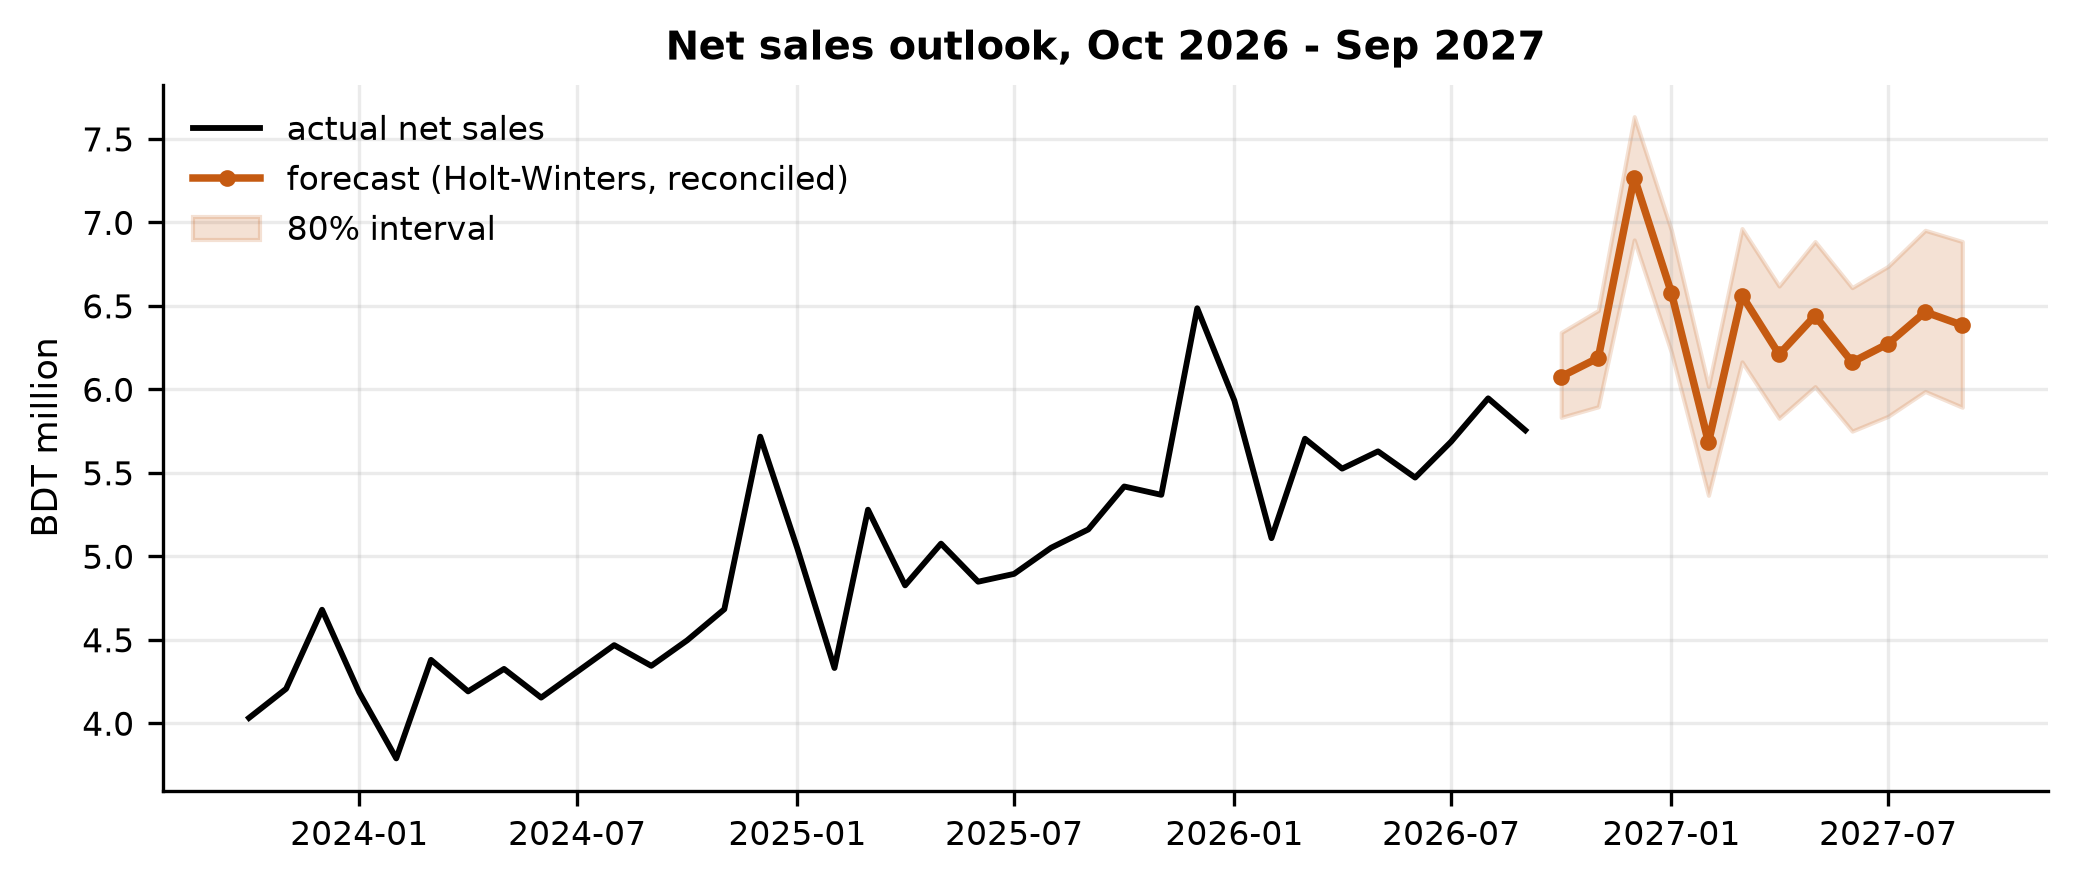
\includegraphics[width=\linewidth]{ml_future_forecast}
\caption{অক্টোবর 2026 -- সেপ্টেম্বর 2027-এর নিট বিক্রয়ের দৃষ্টিভঙ্গি, 80\% পূর্বাভাস-ব্যবধানসহ}\label{fig:future}
\end{figure}

\section{বড় অর্ডারের ক্লাসিফিকেশন}
ক্লাসিফায়ারটি অর্ডার এন্ট্রির সময় পাওয়া তথ্য থেকে অনুমান করে অর্ডারে অন্তত 10 ইউনিট থাকবে কি না। প্রশিক্ষণ-অর্ডারের \ClsPosTrain\% এবং
পরীক্ষা-অর্ডারের \ClsPosTest\% ছিল বড়। মডেলগুলো \ClsTrain টি অর্ডারে (2020--2024) প্রশিক্ষিত এবং \ClsTest টি অর্ডারে (2025--2026)
পরীক্ষিত। ফিচার: চ্যানেল, অঞ্চল, গ্রাহকের ধরন, ক্যাটাগরি, মূল্য, ডিসকাউন্ট, প্যাক সাইজ, পণ্যের বয়স ও ক্যালেন্ডার-চলক, এবং চ্যানেল
$\times$ অঞ্চল ও পণ্যের smoothed target encoding।

\begin{table}[htbp]
\centering
\footnotesize
\caption{বড় অর্ডার ক্লাসিফিকেশন ($\geq$10 ইউনিট): পরীক্ষাকালের কর্মদক্ষতা, 2025--2026}
\label{tab:classification}
\begin{adjustbox}{max width=\linewidth}
\begin{tabular}{lrrrrrrrrr}
\toprule
\textbf{Model} & \textbf{Accuracy} & \textbf{Precision} & \textbf{Recall} & \textbf{F1} & \textbf{ROC-AUC} & \textbf{PR-AUC} & \textbf{Threshold} & \textbf{Lift@10\%} & \textbf{Time (s)} \\
\midrule
Logistic Regression & 0.661 & 0.357 & 0.628 & 0.455 & 0.712 & 0.418 & 0.62 & 2.35 & 15 \\
Support Vector Machine (linear) & 0.629 & 0.341 & 0.698 & 0.458 & 0.711 & 0.417 & 0.31 & 2.34 & 42 \\
Gradient Boosting (hist) & 0.709 & 0.387 & 0.502 & 0.437 & 0.711 & 0.418 & 0.23 & 2.34 & 35 \\
Random Forest & 0.628 & 0.341 & 0.701 & 0.459 & 0.710 & 0.418 & 0.51 & 2.33 & 252 \\
XGBoost & 0.635 & 0.343 & 0.676 & 0.455 & 0.709 & 0.416 & 0.20 & 2.34 & 60 \\
Decision Tree & 0.550 & 0.309 & 0.807 & 0.447 & 0.709 & 0.407 & 0.48 & 2.31 & 14 \\
K-Nearest Neighbors & 0.634 & 0.333 & 0.624 & 0.434 & 0.684 & 0.396 & 0.20 & 2.28 & 73 \\
\bottomrule
\end{tabular}
\end{adjustbox}
\par\smallskip\parbox{0.92\linewidth}{\footnotesize\emph{টীকা:} পরীক্ষা-বছরে বড় অর্ডারের হার: 22.5\%; যে ক্লাসিফায়ার সবসময় `বড় নয়' বলে তার accuracy হতো 77.5\%, তাই কেবল accuracy বিভ্রান্তিকর। Threshold 2024 validation-বছরে F1 সর্বোচ্চ করে। KNN 60,000-সারির প্রশিক্ষণ-নমুনা ব্যবহার করে। Lift@10\% = সর্বোচ্চ স্কোরের 10\% অর্ডারে বড় অর্ডারের হার ভাগ সামগ্রিক হার।}
\end{table}

\Cref{tab:classification} ও \cref{fig:classification} একটি স্পষ্ট ও শিক্ষণীয় ফলাফল দেখায়। সাতটি অ্যালগরিদমেরই ROC-AUC প্রায় সমান,
\ClsAUCmin থেকে \ClsAUC, এবং \ClsBest সেরা। যে মডেল সবসময় ``বড় নয়'' বলে, সেটি \ClsMajority\% নির্ভুল হলেও অকেজো। বিপরীতে টিউন
করা মডেলগুলো বেশিরভাগ বড় অর্ডার খুঁজে পায় (\ClsBest-এর recall প্রায় \ClsRecall) মাঝারি precision-এ, এবং স্কোর অনুযায়ী শীর্ষ 10\%
অর্ডারে বড় অর্ডার গড়ের চেয়ে \ClsLift গুণ বেশি। সীমা নির্ধারণ করছে ডেটায় থাকা \emph{তথ্য}, অ্যালগরিদম নয়: XGBoost (\ClsXGBAUC)
logistic regression-এর চেয়ে কিছুই বাড়ায় না, আর KNN (\ClsKNNAUC) সবচেয়ে দুর্বল, কারণ অনেক one-hot ফিচারে দূরত্ব অর্থহীন হয়ে পড়ে।

\begin{figure}[htbp]\centering
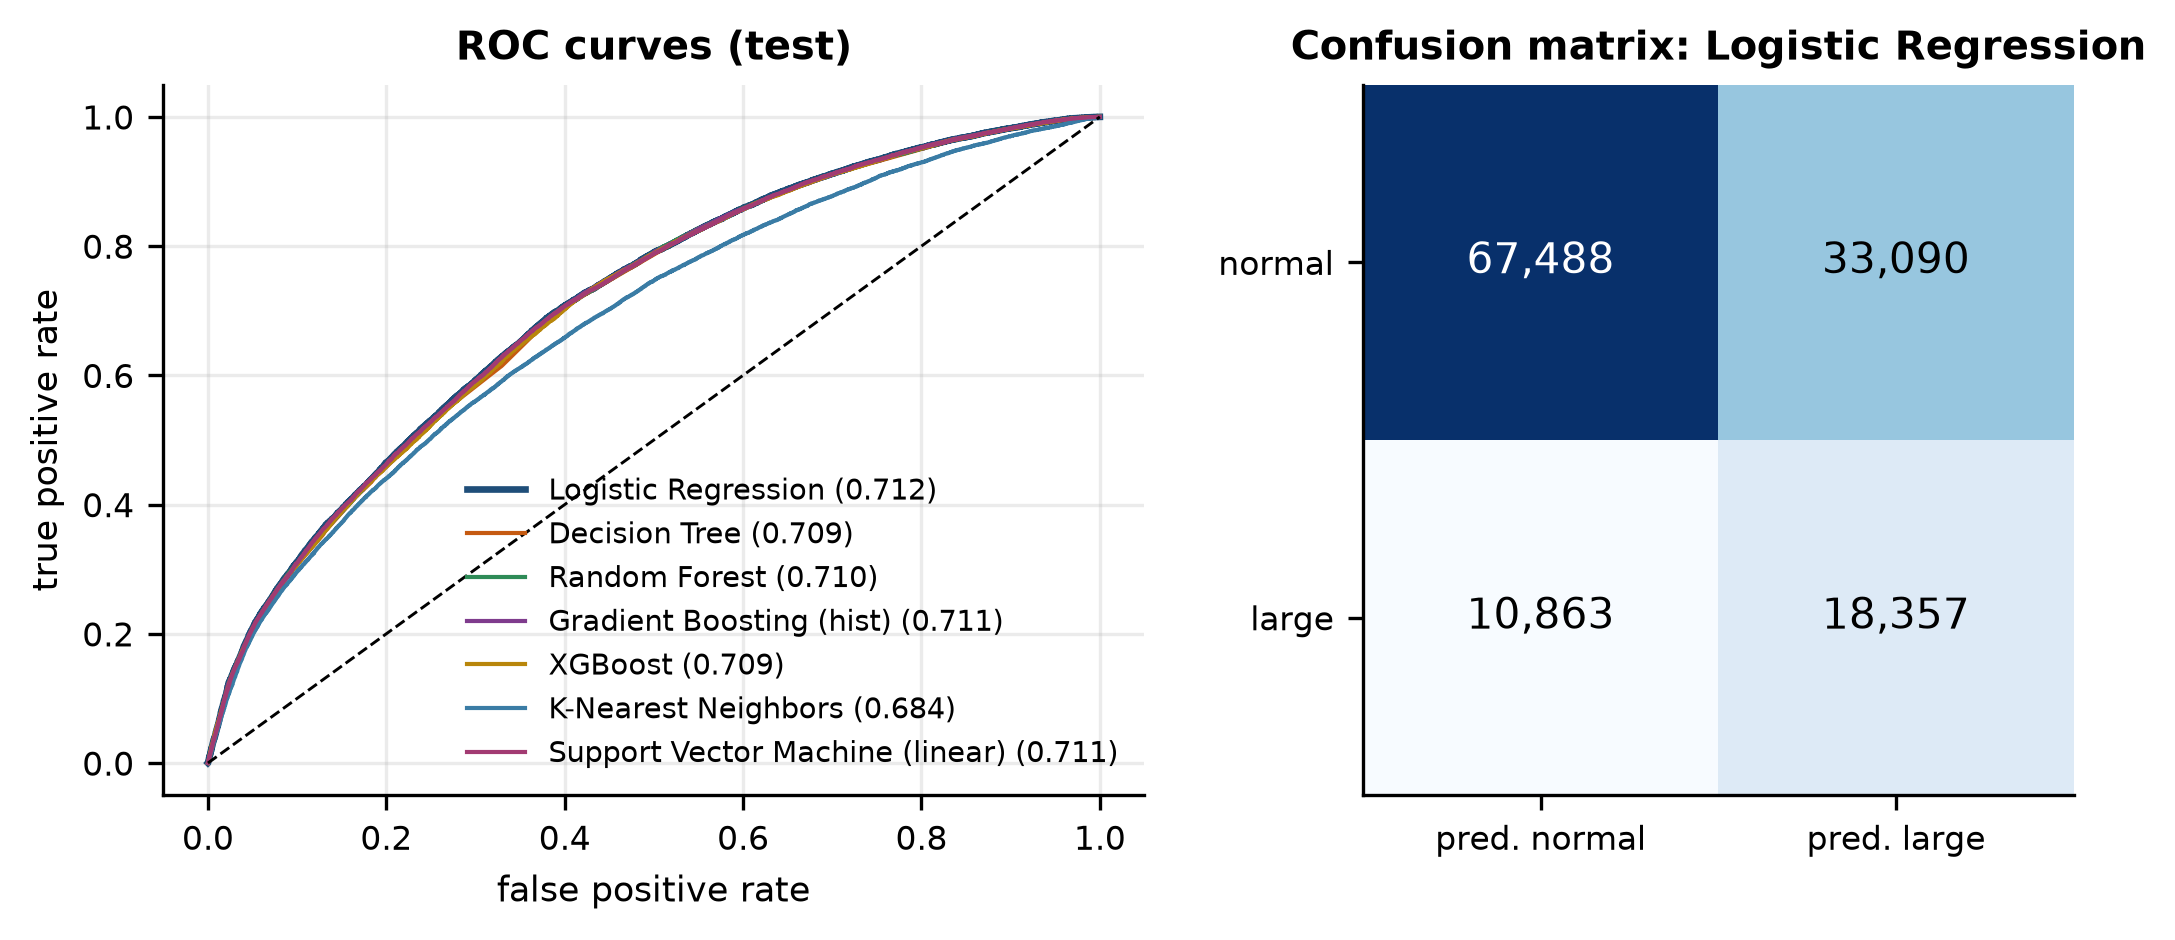
\includegraphics[width=\linewidth]{ml_classification}
\caption{বড় অর্ডার ক্লাসিফিকেশনের ROC বক্ররেখা (বামে), সেরা মডেলের confusion matrix (মাঝে) এবং মেট্রিক তুলনা (ডানে)}\label{fig:classification}
\end{figure}

XGBoost-এর gain importance (\cref{fig:clsimp}) কারণটি চিহ্নিত করে: মডেলের gain-এর প্রায় \ClsChannelImp\% আসে বিক্রয় চ্যানেল থেকে
এবং প্রায় \ClsRegionImp\% অঞ্চল থেকে, আর পণ্য, মূল্য, ডিসকাউন্ট ও ক্যালেন্ডারের অবদান অতি সামান্য। পরীক্ষা-বছরগুলোতে ডিস্ট্রিবিউটর
অর্ডারের \LargeDist\% ছিল বড়, অথচ E-commerce অর্ডারের মাত্র \LargeEcom\%। চ্যানেল ও অঞ্চলের ভেতরে অর্ডারের আকার প্রায় এলোমেলো।
তাই সিদ্ধান্ত গ্রহণে উপযোগী ফল হলো লজিস্টিক পরিকল্পনার জন্য \emph{চ্যানেল-ও-অঞ্চল-স্তরের} বড় অর্ডারের প্রত্যাশা, অর্ডার-বাই-অর্ডার
সুনির্দিষ্ট পূর্বাভাস নয়।

\begin{figure}[htbp]\centering
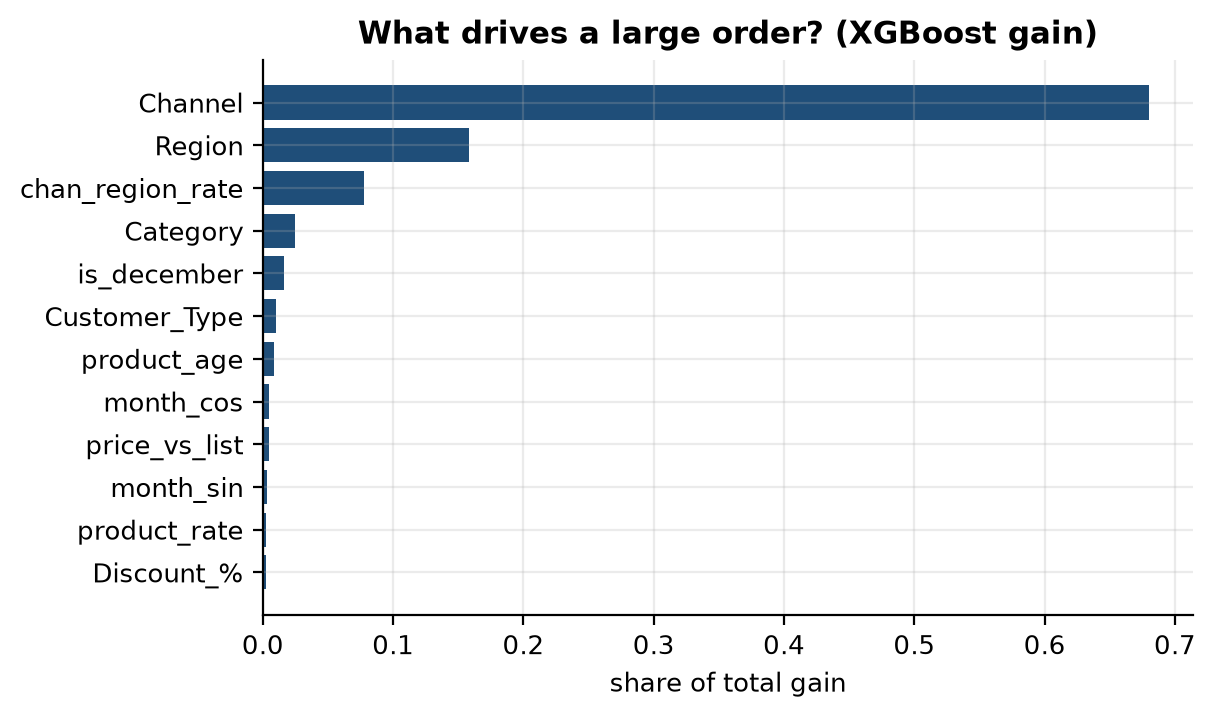
\includegraphics[width=.65\linewidth]{ml_classification_importance}
\caption{বড় অর্ডারের চালিকাশক্তি: মূল চলক অনুযায়ী একত্রিত XGBoost gain}\label{fig:clsimp}
\end{figure}

\section{বিভাজন}
\subsection{পণ্য পোর্টফোলিও}
প্রতিটি পণ্যকে বর্ণনা করা হয়েছে এর log আয়, log গড় মূল্য, 2023 থেকে 2025-এর ইউনিট প্রবৃদ্ধি, ডিসেম্বর মৌসুমি সূচক এবং মাস-থেকে-মাসের
অস্থিরতা দিয়ে। অর্ডারের আকার ও চ্যানেল-মিশ্রণ বাদ দেওয়া হয়েছে, কারণ পণ্যভেদে এগুলো প্রায় একই (\cref{ch:eda}) এবং কেবল noise যোগ
করত। ফিচারগুলো standardise করে $k=2,\dots,8$-এর জন্য $K$-Means, agglomerative (Ward) ও Gaussian-mixture ক্লাস্টারিং তুলনা করা হয়েছে
(\cref{fig:clustering}, \cref{tab:clustercompare})। তিন থেকে পাঁচটি বিভাগের ব্যবহারিক সীমার মধ্যে $k=\ProdK$-এ $K$-Means সেরা silhouette
(\ProdSil) ও Davies--Bouldin সূচক \ProdDB দিয়েছে। ফলস্বরূপ বিভাগগুলো \cref{tab:productclusters}-এ সংক্ষেপিত এবং তাদের গড় থেকে
স্বয়ংক্রিয়ভাবে নামকরণ করা।

\begin{table}[htbp]
\centering
\small
\caption{পণ্য-পোর্টফোলিওর বিভাগ (K-Means, k=5)}
\label{tab:productclusters}
\begin{adjustbox}{max width=\linewidth}
\begin{tabular}{lrrrrrr}
\toprule
\textbf{Segment} & \textbf{Products} & \textbf{Sales share \%} & \textbf{Avg price} & \textbf{Units/order} & \textbf{Unit growth \%/yr} & \textbf{Dec. index} \\
\midrule
Premium \& gift packs & 13 & 33.3 & 156 & 6.24 & +7.8 & 123 \\
Mature slow-growth lines & 13 & 31.9 & 130 & 6.17 & +2.3 & 120 \\
Core family packs & 11 & 28.1 & 133 & 6.17 & +4.9 & 134 \\
Single-serve value packs & 9 & 4.2 & 23 & 6.22 & +6.0 & 119 \\
Niche \& new lines & 6 & 2.5 & 24 & 6.22 & +4.0 & 134 \\
\bottomrule
\end{tabular}
\end{adjustbox}
\par\smallskip\parbox{0.92\linewidth}{\footnotesize\emph{টীকা:} প্রবৃদ্ধি হলো 2023 থেকে 2025-এর মধ্যে ইউনিটের চক্রবৃদ্ধি বার্ষিক হার। ডিসেম্বর সূচক = পণ্যের গড় মাসের তুলনায় গড় ডিসেম্বরের ইউনিট (100 = মৌসুমিতা নেই)।}
\end{table}

\subsection{বাজার-বিভাগ}
অঞ্চল, চ্যানেল ও গ্রাহকের ধরনের 220টি সমন্বয়কে তাদের আয়, গড় অর্ডার-মূল্য, অর্ডারপ্রতি ইউনিট, মূল্য, ডিসকাউন্ট, প্রবৃদ্ধি ও গিফট-প্যাকের
অংশ দিয়ে ক্লাস্টার করা হয়েছে। $K$-Means $k=\MktK$টি বিভাগ বেছে নিয়েছে (silhouette \MktSil), যা স্পষ্টভাবে ভাগ হয়: \emph{core retail
trade} (বড় শহরে General ও Modern Trade), \emph{bulk distribution}, ছোট-অঙ্কের \emph{online ও আঞ্চলিক} কোষ, এবং একদল
\emph{উদীয়মান উচ্চ-প্রবৃদ্ধির} কোষ (\cref{tab:marketclusters})।

\begin{table}[htbp]
\centering
\scriptsize
\caption{অঞ্চল $\times$ চ্যানেল $\times$ গ্রাহকের ধরন কোষের বাজার-বিভাগ (K-Means, k=4)}
\label{tab:marketclusters}
\begin{adjustbox}{max width=\linewidth}
\begin{tabular}{lrrrrrll}
\toprule
\textbf{Segment} & \textbf{Cells} & \textbf{Sales share \%} & \textbf{AOV (BDT)} & \textbf{Units/order} & \textbf{Growth \%/yr} & \textbf{Main channels} & \textbf{Main regions} \\
\midrule
Core retail trade & 99 & 71.9 & 518 & 5.02 & +14.8 & General Trade, Modern Trade & Dhaka, Chattogram, Gazipur \\
Bulk distribution & 52 & 22.6 & 966 & 9.96 & +16.2 & Distributor & Chattogram, Dhaka, Gazipur \\
Small-ticket online \& regional & 50 & 4.2 & 341 & 3.43 & +16.7 & E-commerce, Modern Trade & Barishal, Khulna, Rajshahi \\
Emerging high-growth cells & 19 & 1.3 & 431 & 4.16 & +33.2 & E-commerce, Modern Trade & Cumilla, Khulna, Mymensingh \\
\bottomrule
\end{tabular}
\end{adjustbox}
\end{table}
\begin{table}[htbp]
\centering
\small
\caption{নির্বাচিত ক্লাস্টার-সংখ্যায় ক্লাস্টারিং অ্যালগরিদমগুলোর তুলনা}
\label{tab:clustercompare}
\begin{adjustbox}{max width=\linewidth}
\begin{tabular}{llrrrr}
\toprule
\textbf{Problem} & \textbf{Algorithm} & \textbf{k} & \textbf{Silhouette} & \textbf{Davies-Bouldin} & \textbf{Calinski-Harabasz} \\
\midrule
Products & K-Means & 5 & 0.237 & 1.271 & 16.2 \\
Products & Agglomerative (Ward) & 5 & 0.212 & 1.195 & 14.9 \\
Products & Gaussian Mixture & 5 & 0.233 & 1.237 & 15.3 \\
Market cells & K-Means & 4 & 0.243 & 1.497 & 54.2 \\
Market cells & Agglomerative (Ward) & 4 & 0.250 & 1.467 & 48.9 \\
Market cells & Gaussian Mixture & 4 & 0.165 & 1.753 & 42.4 \\
\bottomrule
\end{tabular}
\end{adjustbox}
\par\smallskip\parbox{0.92\linewidth}{\footnotesize\emph{টীকা:} উচ্চতর silhouette ও Calinski--Harabasz এবং নিম্নতর Davies--Bouldin মান বেশি পৃথক ক্লাস্টার নির্দেশ করে।}
\end{table}

\begin{figure}[htbp]\centering
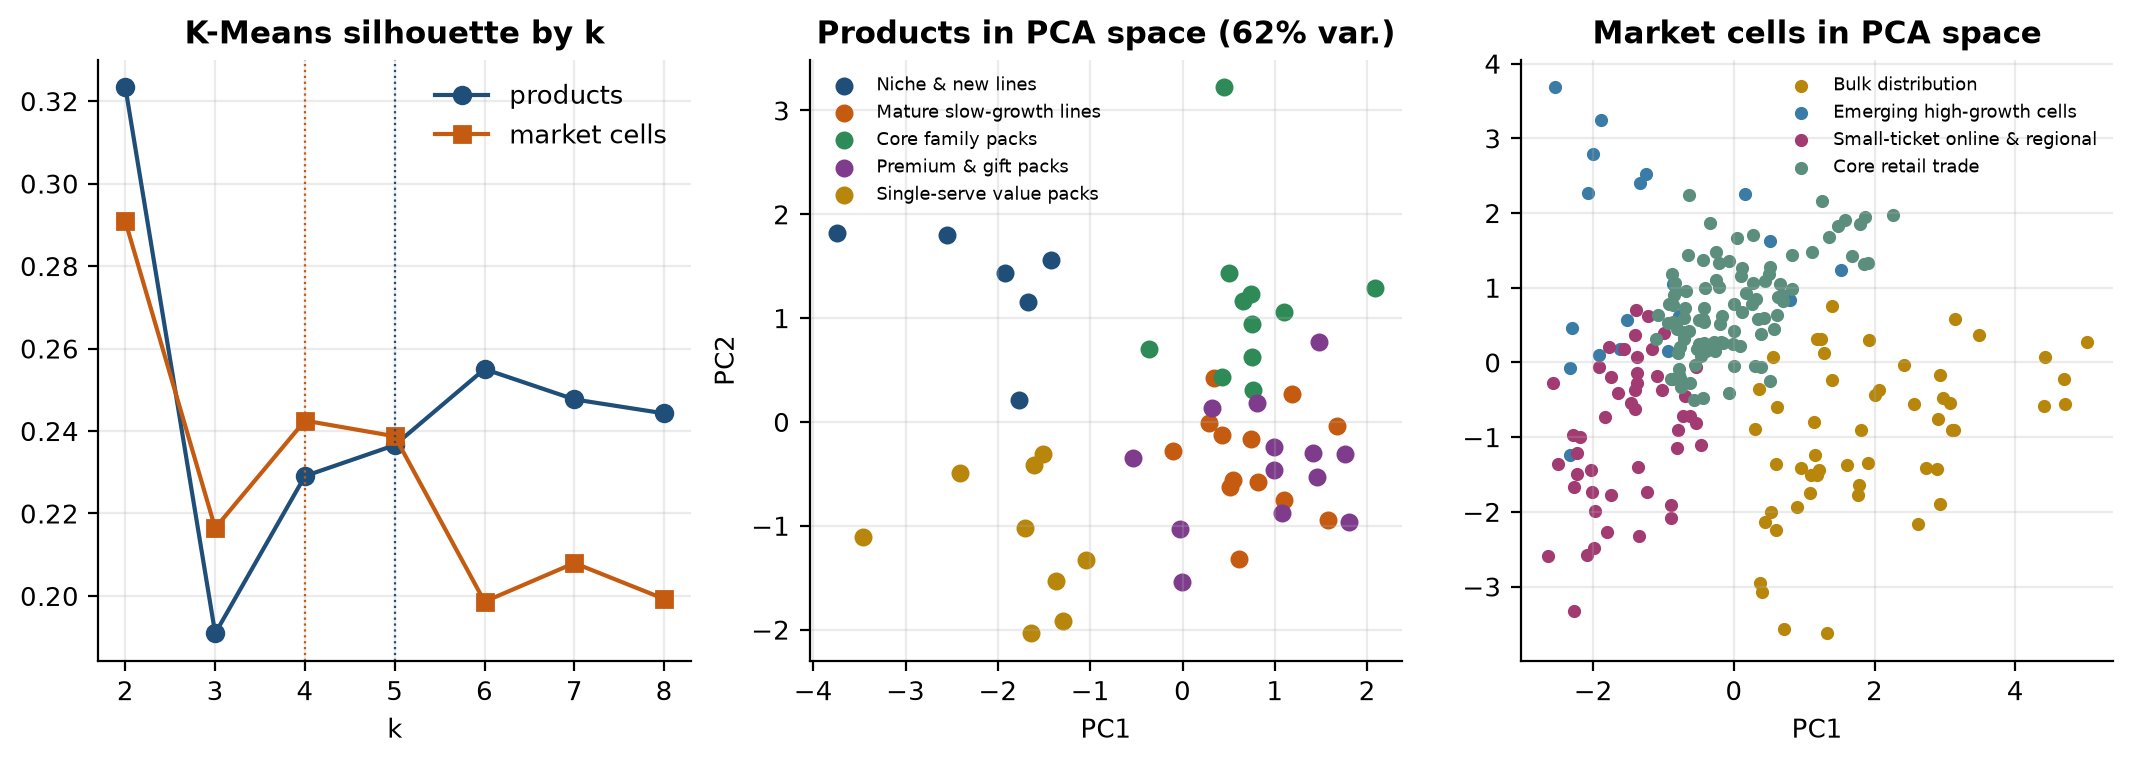
\includegraphics[width=\linewidth]{ml_clustering}
\caption{ক্লাস্টারের সংখ্যা অনুযায়ী silhouette স্কোর (বামে); প্রথম দুটি principal component-এ প্রক্ষিপ্ত পণ্য (মাঝে) ও বাজার-কোষ (ডানে)}\label{fig:clustering}
\end{figure}

Silhouette মান (\ProdSil ও \MktSil) দুর্বল থেকে মাঝারি কাঠামো নির্দেশ করে \citep{rousseeuw1987}। তাই বিভাগগুলো কৌশলের জন্য উপযোগী
সারসংক্ষেপ, স্পষ্টভাবে পৃথক প্রাকৃতিক দল নয়। $K$-Means ও Ward ক্লাস্টারিং প্রায় একমত ছিল, আর এই ছোট নমুনায় Gaussian mixture
সবচেয়ে দুর্বল। পাঠক যাতে বিভাজনের দৃঢ়তা বিচার করতে পারেন, সে জন্য এই ক্রম উল্লেখ করা হলো।

\section{অ্যানোমালি ডিটেকশন}
\subsection{দৈনিক পর্যবেক্ষণ}
প্রতিটি দিনের প্রত্যাশিত মান হিসাব করা হয়েছে একটি 31-দিনের কেন্দ্রীভূত rolling median-কে বছরের মাস অনুযায়ী মৌসুমি গুণক দিয়ে গুণ করে।
বিচ্যুতিগুলো log স্কেলে robust $z$-score $z = 0.6745\,(r-\tilde r)/\text{MAD}$ দিয়ে এবং আলাদাভাবে চারটি দৈনিক ফিচারের উপর একটি
Isolation Forest দিয়ে স্কোর করা হয়েছে। দুটি পদ্ধতি মিলে 2,465টি ব্যবসায়িক দিনের মধ্যে \AnomDays টি চিহ্নিত করেছে: robust $z$-score
দিয়ে \AnomDaysZ টি ও Isolation Forest দিয়ে \AnomDaysIF টি (\cref{fig:anomdaily}, \cref{tab:dailyanom})। বেশিরভাগ চিহ্নিত দিন অস্বাভাবিক
দুর্বল ব্যবসায়িক দিন; বাস্তব প্রয়োগে প্রতিটি দিন সরকারি ছুটি, ধর্মঘট বা সিস্টেম-বিভ্রাটের মতো জানা কারণের সঙ্গে মিলিয়ে দেখা হবে।

\begin{figure}[htbp]\centering
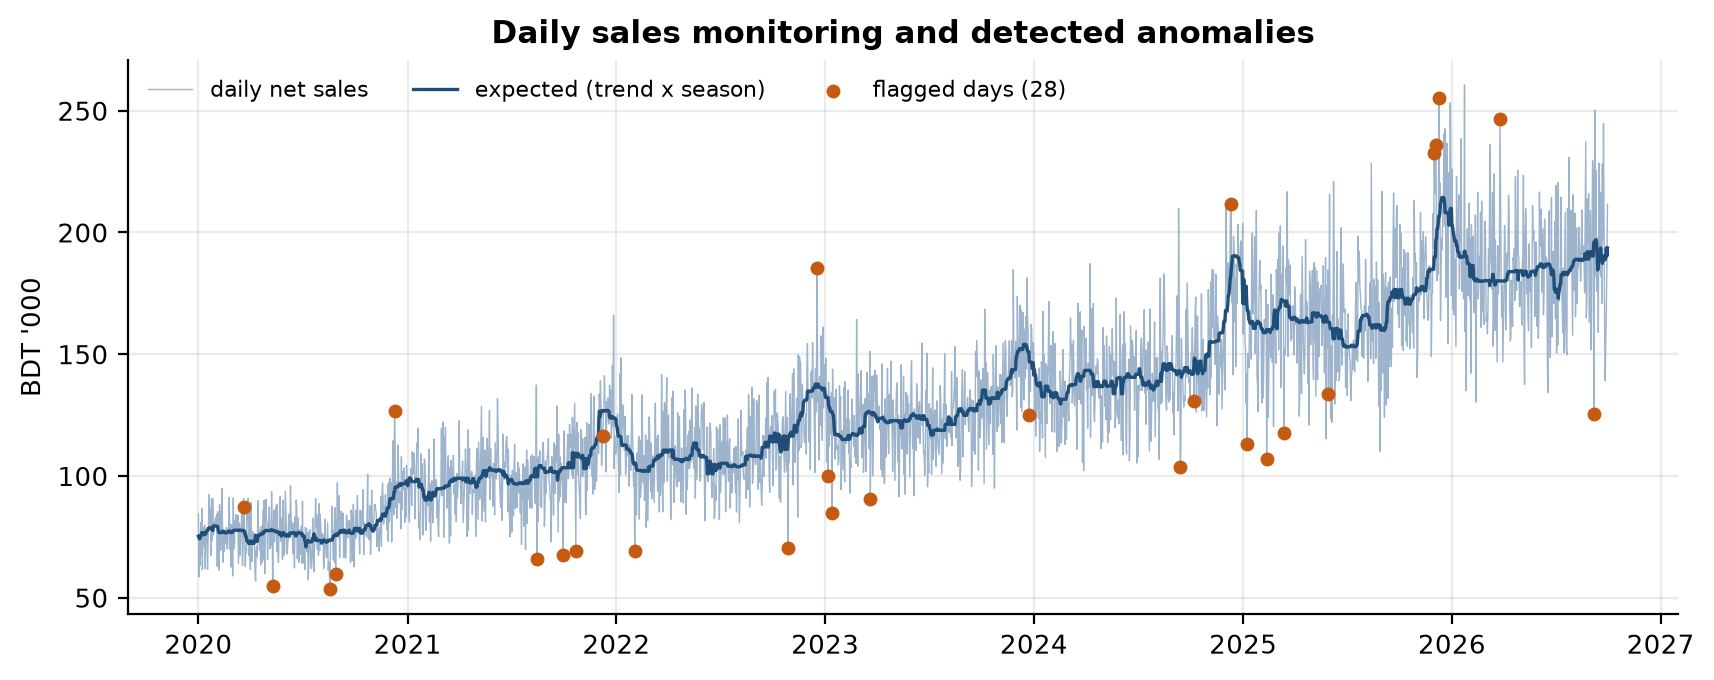
\includegraphics[width=\linewidth]{anomaly_daily}
\caption{দৈনিক নিট বিক্রয়, প্রত্যাশিত স্তর ও শনাক্তকৃত অস্বাভাবিকতা}\label{fig:anomdaily}
\end{figure}
\begin{table}[htbp]
\centering
\small
\caption{দশটি সবচেয়ে অস্বাভাবিক ব্যবসায়িক দিন (মৌসুমি-সমন্বিত)}
\label{tab:dailyanom}
\begin{adjustbox}{max width=\linewidth}
\begin{tabular}{lrrrrl}
\toprule
\textbf{Date} & \textbf{Net sales (BDT)} & \textbf{Expected (BDT)} & \textbf{Deviation \%} & \textbf{Robust z} & \textbf{Flagged by} \\
\midrule
28 Oct 2022 & 70,215 & 113,462 & -38.1 & -4.01 & robust z \\
22 Oct 2021 & 69,194 & 109,276 & -36.7 & -3.82 & robust z \\
06 Sep 2026 & 125,262 & 195,913 & -36.1 & -3.74 & robust z \\
30 Sep 2021 & 67,358 & 103,385 & -34.8 & -3.58 & both \\
02 Feb 2022 & 69,149 & 104,763 & -34.0 & -3.47 & Isolation Forest \\
15 Aug 2021 & 66,039 & 99,664 & -33.7 & -3.44 & Isolation Forest \\
11 Feb 2025 & 106,843 & 160,093 & -33.3 & -3.38 & Isolation Forest \\
13 Jan 2023 & 84,814 & 126,483 & -32.9 & -3.34 & Isolation Forest \\
08 Jan 2025 & 113,188 & 168,043 & -32.6 & -3.31 & Isolation Forest \\
13 Mar 2025 & 117,699 & 171,855 & -31.5 & -3.17 & Isolation Forest \\
\bottomrule
\end{tabular}
\end{adjustbox}
\end{table}

\subsection{লেনদেন যাচাই}
লেবেলযুক্ত ত্রুটি না থাকায় প্রকৃত ডেটায় ডিটেক্টরের সক্ষমতা মাপা যায় না। তাই প্রিপ্রসেসিং স্ক্রিপ্টের পদ্ধতি অনুসরণ করে 500,000 অর্ডারের
একটি অনুলিপিতে চার ধরনের (প্রতিটি 250টি) মোট 1,000টি বাস্তবসম্মত ত্রুটি রোপণ করা হয়েছে (\cref{tab:anomaly})। পরিমাণের উপর প্রতি-পণ্য
IQR নিয়ম রোপিত ত্রুটির মাত্র \AnomIQRRecall\% ধরেছে, কারণ চার ধরনের তিনটিতে পরিমাণ জড়িত নয়। মূল্য ও ডিসকাউন্টের উপর সরল ব্যবসায়িক
নিয়ম নিখুঁত precision-এ \AnomRuleRecall\% ধরেছে, কিন্তু পরিমাণের সব ত্রুটি বাদ পড়েছে। Isolation Forest চার ধরনেই মিলিয়ে \AnomIFRecall\%
ধরেছে: মূল্য ও ডিসকাউন্টের ত্রুটি সম্পূর্ণভাবে, এবং বেশিরভাগ স্ফীত পরিমাণও। শিক্ষা হলো নিয়ম ও মেশিন লার্নিং পরস্পরের পরিপূরক: জানা
ব্যর্থতার ক্ষেত্রে নিয়ম নিখুঁত, আর অজানা ক্ষেত্রে Isolation Forest বিস্তৃত সুরক্ষা দেয়।

\begin{table}[htbp]
\centering
\footnotesize
\caption{500,000 অর্ডারে রোপিত 1,000টি লেনদেন-ত্রুটির শনাক্তকরণ}
\label{tab:anomaly}
\begin{adjustbox}{max width=\linewidth}
\begin{tabular}{lrrrrrrr}
\toprule
\textbf{Method} & \textbf{Flagged} & \textbf{Precision} & \textbf{Recall} & \textbf{Price x10} & \textbf{Qty x20} & \textbf{Disc. 30-45\%} & \textbf{Price 10\%} \\
\midrule
IQR on log quantity (per product) & 1,500 & 0.112 & 0.168 & 0.00 & 0.66 & 0.00 & 0.01 \\
Business rules (price, discount) & 750 & 1.000 & 0.750 & 1.00 & 0.00 & 1.00 & 1.00 \\
Isolation Forest (4 features) & 2,500 & 0.364 & 0.909 & 1.00 & 0.64 & 1.00 & 1.00 \\
Rules OR Isolation Forest & 2,500 & 0.364 & 0.909 & 1.00 & 0.64 & 1.00 & 1.00 \\
\bottomrule
\end{tabular}
\end{adjustbox}
\par\smallskip\parbox{0.92\linewidth}{\footnotesize\emph{টীকা:} শেষ চারটি কলাম দেখায় প্রতিটি ধরনের ত্রুটির কত অংশ শনাক্ত হয়েছে। ডেটার একটি অনুলিপিতে প্রতিটি ধরনের 250টি ত্রুটি রোপণ করা হয়েছে।}
\end{table}

\section{মডেল মূল্যায়নের সারসংক্ষেপ}
\begin{table}[htbp]\centering\small
\caption{প্রতিটি বিশ্লেষণী সমস্যার জন্য নির্বাচিত মডেলের সারসংক্ষেপ}\label{tab:modelsummary}
\begin{tabularx}{\linewidth}{@{}lXl@{}}
\toprule
\textbf{সমস্যা} & \textbf{নির্বাচিত পদ্ধতি} & \textbf{প্রধান পরীক্ষা-ফল} \\ \midrule
পণ্যের চাহিদা (এক-ধাপ) & \BestReg & WAPE \BestRegWAPE\%, $R^2$ \BestRegRtwo \\
পণ্যের চাহিদা (বহু-ধাপ) & \BestRec, recursive & WAPE \BestRecWAPE\% \\
কোম্পানির মোট & Holt--Winters + top-down reconciliation & MAPE \HWMAPE\% \\
বড় অর্ডার & \ClsBest & ROC-AUC \ClsAUC, lift \ClsLift \\
পণ্য-বিভাগ & $K$-Means, $k=\ProdK$ & silhouette \ProdSil \\
বাজার-বিভাগ & $K$-Means, $k=\MktK$ & silhouette \MktSil \\
লেনদেনের অস্বাভাবিকতা & নিয়ম অথবা Isolation Forest & recall \AnomComboRecall\% \\ \bottomrule
\end{tabularx}
\end{table}
প্রস্তাবনার নির্দেশ অনুযায়ী মডেল বাছাই করা হয়েছে উপযুক্ত মেট্রিক \emph{এবং} ব্যবসায়িক প্রাসঙ্গিকতা দিয়ে, কেবল নির্ভুলতা দিয়ে নয়। যেখানে
সরল মডেল জটিল মডেলের সমান কাজ করেছে (যেমন ক্লাসিফিকেশনে logistic regression বনাম XGBoost), সেখানে সরল ও বেশি ব্যাখ্যাযোগ্য মডেলটি
অগ্রাধিকার পেয়েছে।
